\section{Ordering and Asynchrony}

\begin{figure}[t]
  \centering
  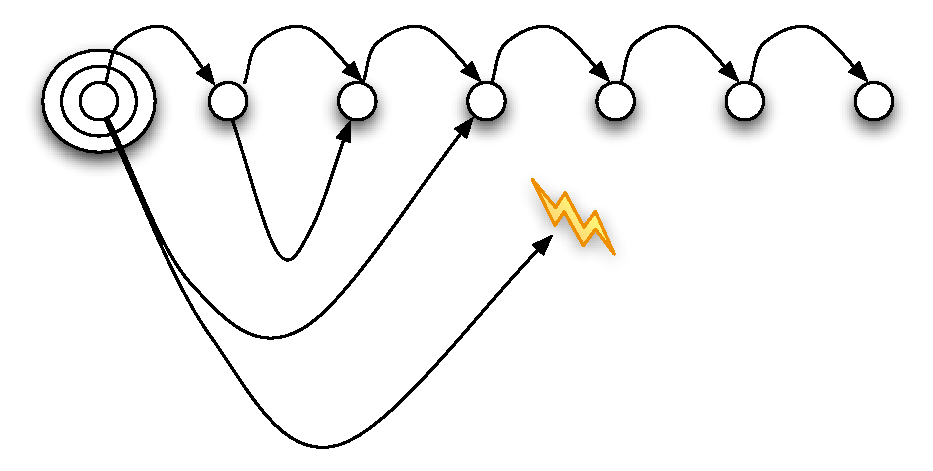
\includegraphics[width=0.75\linewidth]{dedalus-time.pdf}
  \label{fig:dedalus-time}
  \caption{Time moves forward in three ways: across strata, to the next fixpoint, and to some future fixpoint.}
\vspace{-8pt}
\end{figure}

Until now we have restricted our discussion to \slang.  In this section we
consider \lang, a superset of \slang that admits aggregate functions, simple
arithmetic and the \emph{choice} construct.  These constructs will allow us to
express programs that establish or enforce an ordering over inputs, and to
reason about the inherent nondeterminism in communication over unreliable
networks that may delay, lose or reorder the results of logical deductions.

\subsection{Aggregate Functions}

We will consider only the class of \emph{exemplary} aggregate
functions~\cite{tag} -- an exemplary aggregate function's codomains is a subset
of its domain -- and the \emph{count} aggregate, which is expressible using
arithmetic.  We allow an exemplary or count aggregate function $\rho$ to appear
in the head of a deductive rule of the form:

\dedalus{p($A_1 \ldots A_n, \rho(A_{n+1}), \ldots \rho(A_{n+m}$) \(\leftarrow\) 
  $q_1(A_1 \ldots A_n), \ldots q_n(A_1 \ldots A_n$);}

\wrm{so you're saying that we can apply an aggregate multiple times in a single rule, but we can only have one kind of aggregate per rule?}

These functions do not affect the expressivity of the language; we admit them
tosimplify our discussion of ordering.  We note that the \emph{min} function,
which we subsequently use, is expressible in Datalog using negation.

\begin{example}
The query below selects, for each distinct value of the first column of $p$, the minimum 
value of the second column.

\begin{Dedalus}
min_p(A, min<B>) \(\leftarrow\) p(A, B);
\end{Dedalus}

The Datalog program below is equivalent:

\begin{Dedalus}
notmin_p(A, B) \(\leftarrow\) p(A, B), p(A, C), B > C;
  
min_p(A, B) \(\leftarrow\) p(A, B), \(\lnot\)notmin_p(A, B);
\end{Dedalus}
\end{example}

%%\dedalus{r\_pos($A_1$, $A_2$, [...], $A_n$, }

%%$\rho$($A_{n+1}$)}

%%$\rho$($A_{n+2}$), [...] $\rho$($A_{n+m}$)) \(\leftarrow\) r($A_1$, $A_2$, [...], $A_n$);}



\subsection{Choice}

\subsection{Asynchronous Rules}

Recall our use of the distinguished variables $\Tau$ and $S$ to represent the
time suffixes respectively in the body and head of a rule
(Section~\ref{sec:syntaxrestrictions}).
%in our discussion of \slang, representing the time suffixes occuring
%respectively in the body and head of a rule.

We call a rule {\em asynchronous} if the relation between $S$ and $\Tau$ is
unknown.  We model this nondeterminism with the choice construct.

An asynchronous rule has the following subgoals in its body:
\dedalus{successor(\_,S), choose(($\Theta$), (S))}, where $\Theta$ is a vector
containing all variables appearing in the rule body, including $\Tau$.  The
choice subgoal expresses that the rule head may be derived in any time suffix.
%time value
%that appears in the \dedalus{successor} relation.

\wrm{this is a bit of a cop out i think, shouldn't we give an actual form
rather than an example?}
\begin{example}
A well-formed asynchronous \lang rule.

\begin{Dedalus}
asynchronous
r(A, B, S) \(\leftarrow\)
   e(A, B, \(\Tau\)), successor(_, S), choose((A, B), (S));
\end{Dedalus}
\end{example}

We admit a new temporal head annotation to sugar the rule above.  The
identifier \dedalus{async} implies the rule is asynchronous, and stands in for
\dedalus{successor(\_, S), choose(($\Theta$), (S))} in the body.  
%%$N$ is a variable,
%%corresponding to the time suffix $\Tau$ of all predicates in the rule body and
%%optionally referenced in the head.  

The above example expressed using \dedalus{async} is:

\begin{Dedalus}
asynchronous
r(A, B)@async \(\leftarrow\) 
  e(A, B);
\end{Dedalus}



\begin{figure}[t]
  \centering
  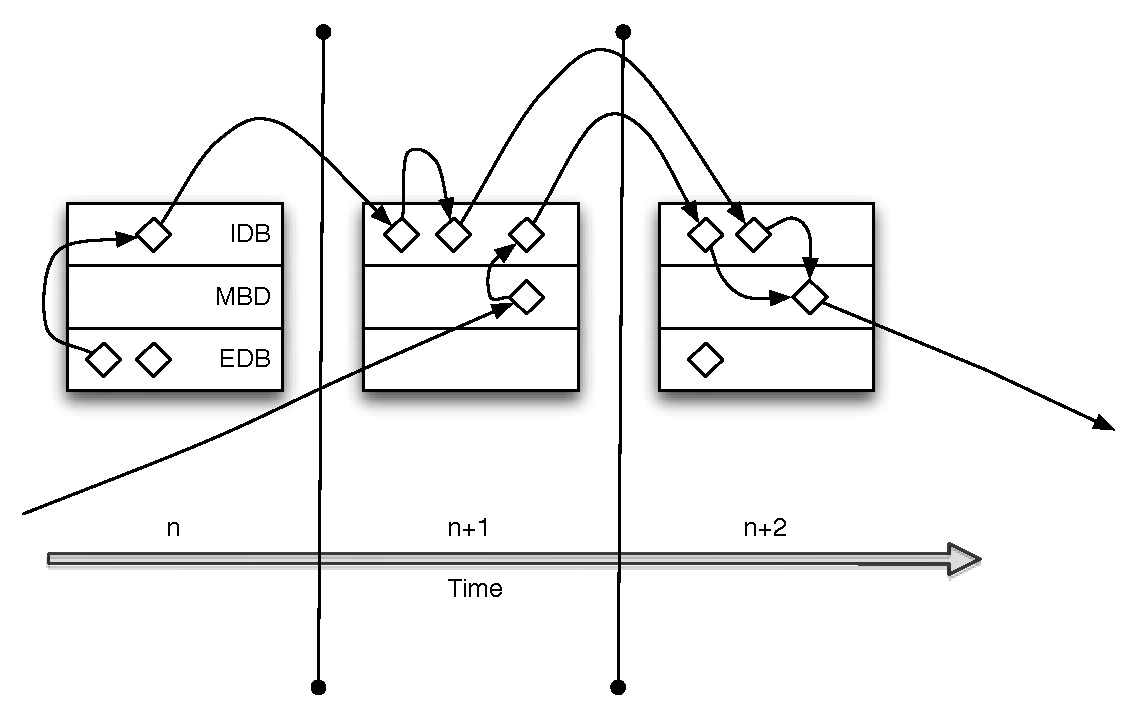
\includegraphics[width=1\linewidth]{edbidbmdb.pdf}
  \label{fig:edbidbmdb}
  \caption{Derivations across time in IDB and MDB relations.}
\vspace{-8pt}
\end{figure}



\subsection{Queues}

%%Consider a trace of events to a 
Consider a predicate \dedalus{balance\_update} that represents updating the a
user's account balance.  Its attributes are a string representing a user, a
floating point number indicating a new account balance and an integer
indicating the order in which the updates were issued, according to some
external clock or sequence:

\begin{Dedalus}
balance\_update("bob", 100.00, 2355)@123;
balance\_update("bob", 75.00, 2358)@123;
balance\_update("alice", 0.00, 2377)@123;
balance\_update("bob", 10.00, 2455)@123;
\end{Dedalus}

Note that all the time suffixes are the same.  
%Depending on the program that implements the balance update, several behaviors
%are possible.
Given this schema, we note that a program would likely want to process
\dedalus{balance\_update} events individually in a data-dependent order, in
spite of their coincidence in logical time.  It is difficult to express general
in-order tuple processing in Datalog, in part because the language does not
admit sequences.
%above is really what we want to say, right? -wrm
%has so
%notion of order of evaluation (except the implicit ordering implied by
%stratification).

In the program below, we define a table \dedalus{m\_balance\_update} that
serves as a queue to feed \dedalus{balance\_update}.  The queue must persist
across timesteps because it may take multiple timesteps to drain it.  At each
fixpoint, for each value of \textbf{A}, a single tuple is projected into
\dedalus{balance\_update} and atomically deleted from
\dedalus{m\_balance\_update}, changing the value of the aggregate calculated at
the subsequent step: \wrm{as opposed to non-atomic deletion? what's that?}

\begin{Dedalus}

m\_balance\_update(A, B, C)@next \(\leftarrow\)
  m\_balance\_update(A, B, C),
  notin del\_m\_balance\_update(A, B, C);

omin(A, min<C>) \(\leftarrow\)
  m\_balance_update(A, _, C);

p(A, B, C)@next \(\leftarrow\)
  m\_balance\_update(A, B, C),
  omin(A, C);

del\_m\_balance\_update(A, B, C) \(\leftarrow\)
  m\_balance\_update(A, B, C),
  omin(A, C);
\end{Dedalus}

Under such a queueing discipline, deductive rules that depend on
\emph{balance\_update} are constrained to consider only one tuple per fixpoint
per value of the variable \textbf{A}, thus implementing a per-user FIFO
discipline.  To enforce a global FIFO ordering over \emph{balance\_update}, we
may redefine \emph{omin} and any dependent rules to exclude the \textbf{A}
atttribute.

A queue establishes a mapping between the local clock and the ordering domain of the input relation. By doing so, we are able to take
advantage of the natural ordering enforced by stratification over time, to enforce an ordering property over our input that is otherwise 
very difficult to express in a logic language.

\wrm{===stopped reading here===}

\subsection{Lamport Clocks}

Implementing a Lamport Clock~\cite{timeclocks} is a special case of a queueing discipline as defined above.
Consider a predicate{m\_balance\_update} as defined above, but with an extra integer attribute that contains the logical transmission
time of the sender (via a message rule) of a given tuple.  For example, the sender's rule will look like: 

\paa{damn it!  we've sugared out N from the syntax!! now what?}

\begin{Dedalus}
entangle
m\_balance\_update(A, B, N)@async \(\leftarrow\)
  send\_p(A, B)@N;
\end{Dedalus}

Note that in the rule named \emph{entangle}, the time suffix is projected into the last attribute of \emph{m\_p}.  
This establishes an \emph{entanglement} between
the sender's local clock and the program dataflow.  The queueing discipline that implements a
Lamport clock is then:

\begin{Dedalus}

m\_balance\_update(A, B, C)@next \(\leftarrow\)
  m\_balance\_update(A, B, C),
  \(\lnot\) del\_m\_balance\_update(A, B, C);

omin(A, min<C>) \(\leftarrow\)
  m\_balance\_update(A, _, C);

lmax(max<C>) \(\leftarrow\)
  m\_balance\_update(_, _, C);

disentangle
balance_update(A, B)next \(\leftarrow\)
  m\_balance\_update(A, B, C)@N,
  omin(A, C)@N,
  lmax(L)@N,
  N > L;

del\_m\_balance\_update(A, B) :-
  m\_balance\_update(A, B),
  omax(B);
  
\end{Dedalus}

Note that the rule named \emph{disentangle} references the data elements $C$ and $L$, both of which
contain timestamps, and induces a \emph{balance\_update} tuple with timestamp $N+1$ only when $N > L$,
the highest of the timestamps in its message queue.  Under the distributed systems model of Lamport clocks, 
we expect the tuples in the message queue to  be from other hosts with independent clocks, sending messages 
over a medium that can delay or reorder them arbitrarily.  In order to make the necessary comparison between local
and remote clocks, it is necessary to reference the time suffix variable directly, rather than omitting it as we have done 
in all other Dedalus examples.

\subsection{Trace Entanglement}

